%%%%%%%%%%%%%%%%%%%%%%%%%%%%%%%%%%%%%%%%%%%%%%%%%%%%%%%%%
\begin{frame}[fragile]{음영 계산의 필요성}

\begin{itemize}
\item 음영(陰影) 계산, 혹은 셰이딩(shading)은 어떤 물체의 표면에서 어두운 부분과 밝은 부분을 서로 다른 밝기로 그려내는 것
\item 모든 면을 동일한 색으로 그리면 입체감이 없다.
\end{itemize}

\begin{figure}[h!]
  \centering
    
\includegraphics[height=4cm]{Math_lighting/shading.png}
\end{figure}

\end{frame}
%%%%%%%%%%%%%%%%%%%%%%%%%%%%%%%%%%%%%%%%%%%%%%%%%%%%%%%%%

%%%%%%%%%%%%%%%%%%%%%%%%%%%%%%%%%%%%%%%%%%%%%%%%%%%%%%%%%
\begin{frame}[fragile]{조명과 재질}

음영 계산에 필요한 두 가지 핵심 요소
\begin{itemize}
\item 빛
	\begin{itemize}
	\item 컴퓨터 그래픽스의 최종 결과는 우리의 눈을 통해 입력되는 시각 정보
	\item 눈이 인지하는 신호는 전자기파
	\item 우리가 인지할 수 있는 영역의 전자기파: 가시광선(可視光線)
	\item 이 가시광선을 일상적으로 `빛'이라 부름
	\end{itemize}
\item 재질(材質,material)
	\begin{itemize}
	\item 같은 빛이라고 모든 물체가 같은 색으로 보이지는 않음
	\item 물체는 저마다의 특성에 따라 서로 다른 방식으로 빛을 반사
	\item 물체가 가진 반사 특성을 재질이라고 함
	\end{itemize}
\end{itemize}

\end{frame}
%%%%%%%%%%%%%%%%%%%%%%%%%%%%%%%%%%%%%%%%%%%%%%%%%%%%%%%%%

%%%%%%%%%%%%%%%%%%%%%%%%%%%%%%%%%%%%%%%%%%%%%%%%%%%%%%%%%
\begin{frame}[fragile]{지역조명과 전역조명}

\begin{figure}[h!]
  \centering
    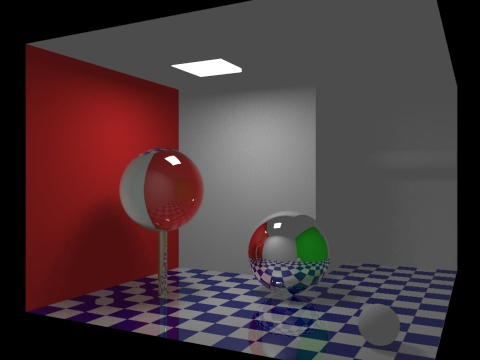
\includegraphics[height=4cm]{Math_lighting/local_illumination.jpg}
    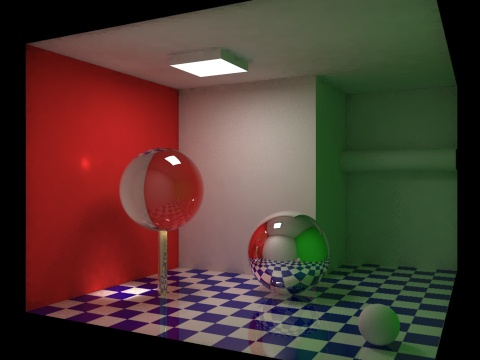
\includegraphics[height=4cm]{Math_lighting/global_illumination.jpg}
\end{figure}

\end{frame}
%%%%%%%%%%%%%%%%%%%%%%%%%%%%%%%%%%%%%%%%%%%%%%%%%%%%%%%%%


%%%%%%%%%%%%%%%%%%%%%%%%%%%%%%%%%%%%%%%%%%%%%%%%%%%%%%%%%
\begin{frame}[fragile]{광원 모델}

일반적인 광원(光源, light source)은 다루기가 쉽지 않다. 하나의 광원은 일정한 면적이나 체적을 가지기 때문에 이 광원에서 나온 빛들을 적분해야 한다.
실제 실시간 렌더링에서는 광원을 하나의 점이나 방향으로 보는 단순화된 모델을 사용한다. 사용되는 광원은 다음과 같은 것들이 있다.

\begin{center}
    \begin{tabular}{ |l| p{12cm} |}
    \hline
    {\small \sf \bf 광원 종류} & {\small \sf \bf 특징} \\ \hline
    {\small \sf 점광원} & {\small \sf 광원의 위치와 색으로 결정. 전방향(omnidirection)으로 빛 진행.}\\ \hline
    {\small \sf 집중광원 } & {\small \sf 점광원에서 일부 입체각으로 빛을 제한.}\\ \hline
    {\small \sf 방향광원 } & {\small \sf 특정한 위치가 아니라 방향에 광원 존재.} \\ \hline
    {\small \sf 주변광원 } & {\small \sf 모든 곳에 동일하게 가해지는 빛.}\\ \hline
    \end{tabular}
\end{center}

\end{frame}
%%%%%%%%%%%%%%%%%%%%%%%%%%%%%%%%%%%%%%%%%%%%%%%%%%%%%%%%%


%%%%%%%%%%%%%%%%%%%%%%%%%%%%%%%%%%%%%%%%%%%%%%%%%%%%%%%%%
\begin{frame}[fragile]{지역 조명 모델 - 퐁(Phong) 모델}

정반사와 난반사, 주변광 반사 특성을 표현할 수 있는 간단하고 빠른 모델

다음과 같은 정보가 필요

\begin{itemize}
\item 광원으로 향하는 벡터 $\mathbf L$
\item 카메라(시점)을 향하는 벡터 $\mathbf E$
\item 법선 벡터 $\mathbf N$
\item 이상적인 반사 방향 $\mathbf R$
\end{itemize}


\begin{figure}[h!]
  \centering
    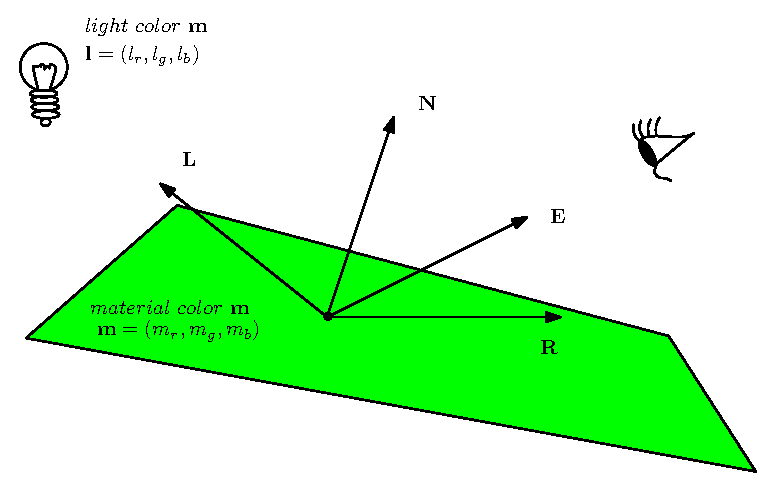
\includegraphics[height=4cm]{Math_lighting/lightingVectors.eps}
\end{figure}

\end{frame}
%%%%%%%%%%%%%%%%%%%%%%%%%%%%%%%%%%%%%%%%%%%%%%%%%%%%%%%%%

%%%%%%%%%%%%%%%%%%%%%%%%%%%%%%%%%%%%%%%%%%%%%%%%%%%%%%%%%
\begin{frame}[fragile]{퐁(Phong) 모델: 광원과 재질 - 색상}

\begin{itemize}
\item 퐁 모델은 난반사, 정반사, 주변광을 각각 독립적으로 계산하여 합성
\item 각각의 반사 요소에 따라 결정해야 하는 것은 눈을 향해 오는 빛의 강도(intensity)와 색상
\item 색상의 결정
	\begin{itemize}
	\item 어떤 광원에서 나오는 빛의 색상이 ${\mathbf l} = (l_r, l_g, l_b)$
	\item 물체의 재질 색상이 ${\mathbf m} = (m_r, m_g, m_b)$
	\item 빛의 색상은 이 빛이 눈에 감지되었을 때 우리가 느끼는 색이
	\item 빨간 색을 가진 물체의 재질 색상 (1.0, 0.0, 0.0)은 도착하는 빛의 RGB 3 개 채널에서 R 채널의 빛을 100\% 반사한다는 것을 의미
	\end{itemize}
\end{itemize}

반사되는 빛의 색상은 다음과 같다.

$$\mathbf c = (l_r m_r, l_g m_g, l_b m_b)$$

이를 이렇게 표현한다.

$$\mathbf c = \mathbf l \otimes \mathbf m $$

\end{frame}
%%%%%%%%%%%%%%%%%%%%%%%%%%%%%%%%%%%%%%%%%%%%%%%%%%%%%%%%%


%%%%%%%%%%%%%%%%%%%%%%%%%%%%%%%%%%%%%%%%%%%%%%%%%%%%%%%%%
\begin{frame}[fragile]{퐁(Phong) 모델: 광원과 재질 - 광강도}

\begin{itemize}
\item 이 계산은 눈에 감지되는 빛의 색상을 결정
\item 같은 색상이라도 밝고 어두울 수 있음
\item 이러한 음영을 고려해야 입체적인 물체로 보임
\item 이러한 음영은 광강도(光强度, light intensity)에 의해 결정
\item 이 광강도의 값은 스칼라(scalar) 값으로 $I$로 표현
\item 실제로 눈에 보이는 색은 광원과 재질에 의해 결정되는 색상 $\mathbf c$와 광강도 $I$에 의해 다음과 같이 결정
\end{itemize}

$$\kappa = I \mathbf c$$

\end{frame}
%%%%%%%%%%%%%%%%%%%%%%%%%%%%%%%%%%%%%%%%%%%%%%%%%%%%%%%%%

%%%%%%%%%%%%%%%%%%%%%%%%%%%%%%%%%%%%%%%%%%%%%%%%%%%%%%%%%
\begin{frame}[fragile]{퐁(Phong) 모델: 최종 결정 반사색}

\begin{itemize}
\item 퐁 모델은 각각의 반사 요소를 모두 따로 계산
\item 난반사 요소와 관련된 값에는 아래첨자 d
\item 정반사에는 s
\item 주변광 반사에는 a
\item 눈에 관측되는 색상은 다음과 같음
\end{itemize}

\begin{eqnarray}
\kappa & = & I_a \mathbf c_a + I_d \mathbf c_d + I_s \mathbf c_s \nonumber
\end{eqnarray}

이때, 주변광의 광강도는 상수 값을 가지므로 $I_a$는 1로 설정할 수 있다. 따라서 다음 식으로 바꿀 수 있다.

\begin{eqnarray} \nonumber
\kappa & = & \mathbf c_a + I_d \mathbf c_d + I_s \mathbf c_s \\ \nonumber 
&  =  & \mathbf l_a \otimes \mathbf m_a + I_d \mathbf l_d \otimes \mathbf m_d + I_s \mathbf l_s \otimes \mathbf m_s \nonumber
\end{eqnarray}

\end{frame}
%%%%%%%%%%%%%%%%%%%%%%%%%%%%%%%%%%%%%%%%%%%%%%%%%%%%%%%%%

%%%%%%%%%%%%%%%%%%%%%%%%%%%%%%%%%%%%%%%%%%%%%%%%%%%%%%%%%
\begin{frame}[fragile]{퐁 모델 광강도(intensity)의 계산 - 난반사}

\begin{itemize}
\item 퐁 모델에서 계산해야 하는 광강도는 난반사 $I_d$와 정반사 $I_s$
\item 난반사는 모든 방향에 동등하게 빛이 퍼지는 것으로 가정
\item 눈이 어디에 있든지 동일한 색상 관찰
\item 눈의 움직임에 따라 변하는 하일라이트(highlight)는 표현하지 못 함
\item 색을 칠하려고 하는 한 지점에 대해 어디서 쳐다 보든지 동일한 밝기
\item 밝기는 얼마나 많은 에너지가 해당 지점에 떨어지는지에 달려 있음
\end{itemize}

\begin{figure}[h!]
  \centering
    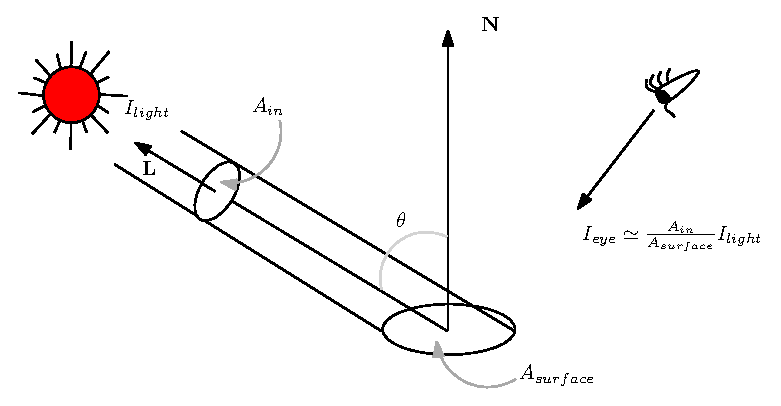
\includegraphics[height=4cm]{Math_lighting/diffuseConcept.eps}
\end{figure}


\end{frame}
%%%%%%%%%%%%%%%%%%%%%%%%%%%%%%%%%%%%%%%%%%%%%%%%%%%%%%%%%

%%%%%%%%%%%%%%%%%%%%%%%%%%%%%%%%%%%%%%%%%%%%%%%%%%%%%%%%%
\begin{frame}[fragile]{퐁 모델 광강도(intensity)의 계산 - 난반사 1/2}

\begin{itemize}
\item 퐁 모델에서 계산해야 하는 광강도는 난반사 $I_d$와 정반사 $I_s$
\item 난반사는 모든 방향에 동등하게 빛이 퍼지는 것으로 가정
\item 눈이 어디에 있든지 동일한 색상 관찰
\item 눈의 움직임에 따라 변하는 하일라이트(highlight)는 표현하지 못 함
\item 색을 칠하려고 하는 한 지점에 대해 어디서 쳐다 보든지 동일한 밝기
\item 밝기는 얼마나 많은 에너지가 해당 지점에 떨어지는지에 달려 있음
\end{itemize}

\begin{figure}[h!]
  \centering
    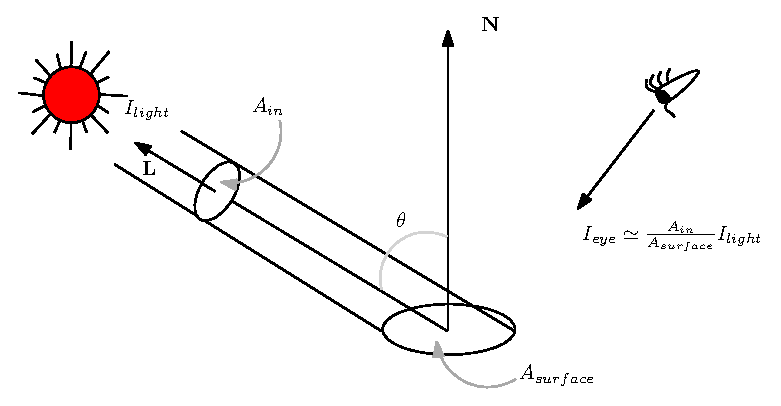
\includegraphics[height=4cm]{Math_lighting/diffuseConcept.eps}
\end{figure}


\end{frame}
%%%%%%%%%%%%%%%%%%%%%%%%%%%%%%%%%%%%%%%%%%%%%%%%%%%%%%%%%

%%%%%%%%%%%%%%%%%%%%%%%%%%%%%%%%%%%%%%%%%%%%%%%%%%%%%%%%%
\begin{frame}[fragile]{퐁 모델 광강도(intensity)의 계산 - 난반사 2/2}

\begin{itemize}
\item 이 값은 광원 벡터 $\mathbf L$과 법선 벡터 $\mathbf N$이 일치할 때 최대이며, 90도를 이룰 때 0이 됨
\item 이 값은 두 벡터의 내적, 즉 두 벡터 사잇각의 코사인(cosine)에 비례한다는 것이 램버트 반사(Lambertian reflectance) 모델
\item 따라서 광강도를 계산해야하는 지점에서 빛을 향하는 방향벡터 $\mathbf L$과 표면 법선벡터 $\mathbf N$의 내적으로  $I_d$를 구할 수 있음
\end{itemize}

\begin{eqnarray}
\label{eq:diffuseIntensity}
I_d  =  \cos \theta   = \mathbf L \cdot \mathbf N
\end{eqnarray}

\end{frame}
%%%%%%%%%%%%%%%%%%%%%%%%%%%%%%%%%%%%%%%%%%%%%%%%%%%%%%%%%


%%%%%%%%%%%%%%%%%%%%%%%%%%%%%%%%%%%%%%%%%%%%%%%%%%%%%%%%%
\begin{frame}[fragile]{퐁 모델 광강도(intensity)의 계산 - 정반사 1/2}

\begin{figure}[h!]
  \centering
    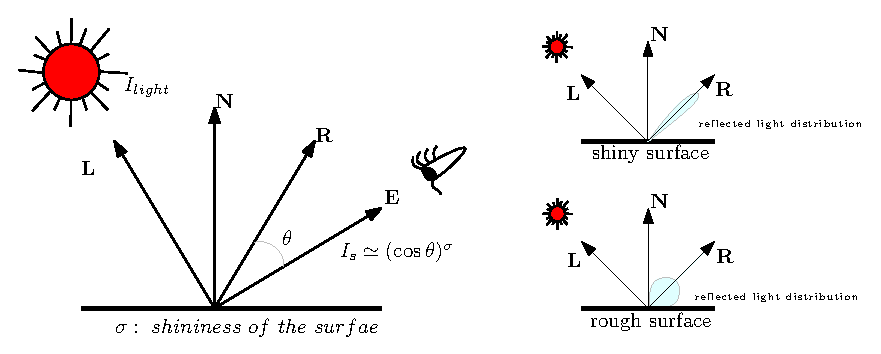
\includegraphics[height=4cm]{Math_lighting/specularConcept.eps}
\end{figure}

정반사는 거울과 같이 입사각에 대칭되는 방향으로 반사되는 것이다. 그런데, 실제 물체들은 이런 이상적인 정반사가 아니라 반사 방향으로 빛이 강하게 진행하기는 하지만 다른 방향으로 조금씩 빛이 나간다. 퐁 모델에서 사용하는 정반사 모델은 거울과 같은 반사가 아니라 반사 벡터 $\mathbf R$ 중심으로 퍼지는 반사를 표현한다.

\end{frame}
%%%%%%%%%%%%%%%%%%%%%%%%%%%%%%%%%%%%%%%%%%%%%%%%%%%%%%%%%

%%%%%%%%%%%%%%%%%%%%%%%%%%%%%%%%%%%%%%%%%%%%%%%%%%%%%%%%%
\begin{frame}[fragile]{퐁 모델 광강도(intensity)의 계산 - 정반사 2/2}

\begin{itemize}
\item 정반사는 반사 벡터 $\mathbf R$ 근처에서 강하게 관찰되기 때문에 눈을  $\mathbf R$ 근처로 가져가야 강한 반사
\item 정반사의 광강도 $I_s$는 $\mathbf R$과 $\mathbf E$의 사잇각의 코사인에 연관
\item 물체의 재질에 따라 $\mathbf R$ 방향으로 집중되는 정도가 달라짐 - 물체의 반질함(shininess) $\sigma$에 의해 결정
\end{itemize}

\begin{eqnarray}
\label{eq:specularIntensity}
I_d  = \cos \theta =  (\mathbf R \cdot \mathbf E )^\sigma \nonumber
\end{eqnarray}

\end{frame}
%%%%%%%%%%%%%%%%%%%%%%%%%%%%%%%%%%%%%%%%%%%%%%%%%%%%%%%%%


%%%%%%%%%%%%%%%%%%%%%%%%%%%%%%%%%%%%%%%%%%%%%%%%%%%%%%%%%
\begin{frame}[fragile]{퐁 모델 광강도(intensity)의 계산 - 주변광}

주변광의 광강도는 언제나 1이다. 따라서 모든 물체는 주변광과 주변광 반사 재질에 의한 색상
$\mathbf l_a \otimes \mathbf m_a$을 기본적으로 갖게 된다.  이것은 지역조명 기법의 단점인 지나치게 어두운 부분을 없애는 역할을 수행한다.

\begin{eqnarray} \nonumber
\kappa & = & \mathbf c_a + I_d \mathbf c_d + I_s \mathbf c_s \\ \nonumber 
&  =  & \mathbf l_a \otimes \mathbf m_a + I_d \mathbf l_d \otimes \mathbf m_d + I_s \mathbf l_s \otimes \mathbf m_s \nonumber
\end{eqnarray}

\end{frame}
%%%%%%%%%%%%%%%%%%%%%%%%%%%%%%%%%%%%%%%%%%%%%%%%%%%%%%%%%

%%%%%%%%%%%%%%%%%%%%%%%%%%%%%%%%%%%%%%%%%%%%%%%%%%%%%%%%%
\begin{frame}[fragile]{수정된 퐁 모델 - 블린(Blinn) 모델}

\begin{itemize}
\item 퐁 모델은 정반사 광강도 계산에서 반사 벡터 $\mathbf R$을 계산해야 함
\item 블린(Blinn)은 이 반사벡터 대신에 반 벡터(halfway vector)라는 것을 도입
\item 반 벡터 $\mathbf H$는 광원 벡터와 시선 벡터 $\mathbf E$를 더해서 정규화: $\mathbf H = \frac{\mathbf L + \mathbf E}{|\mathbf L + \mathbf E|}$
\end{itemize}

\begin{figure}[h!]
  \centering
    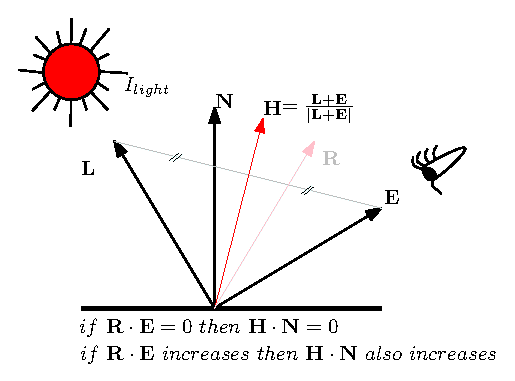
\includegraphics[height=5cm]{Math_lighting/halfwayVector.eps}
\end{figure}

\begin{eqnarray}
\kappa  =  \mathbf l_a \otimes \mathbf m_a + (\mathbf L \cdot \mathbf N) \mathbf l_d \otimes \mathbf m_d + 
(\mathbf H \cdot \mathbf N )^\sigma \mathbf l_s \otimes \mathbf m_s \nonumber
\end{eqnarray}


\end{frame}
%%%%%%%%%%%%%%%%%%%%%%%%%%%%%%%%%%%%%%%%%%%%%%%%%%%%%%%%%

%%%%%%%%%%%%%%%%%%%%%%%%%%%%%%%%%%%%%%%%%%%%%%%%%%%%%%%%%
\begin{frame}[fragile]{구로(Gouraud) 세이딩}

\begin{itemize}
\item 각 정점에 법선 벡터 정의
\item 법선 벡터와 조명의 관계를 이용하여 정점별 퐁 쉐이딩
\item 정점의 색을 이용하여 내부의 픽셀은 선형보간(linear interpolation)을 통해 얻음
\end{itemize}

\begin{figure}[h!]
  \centering
    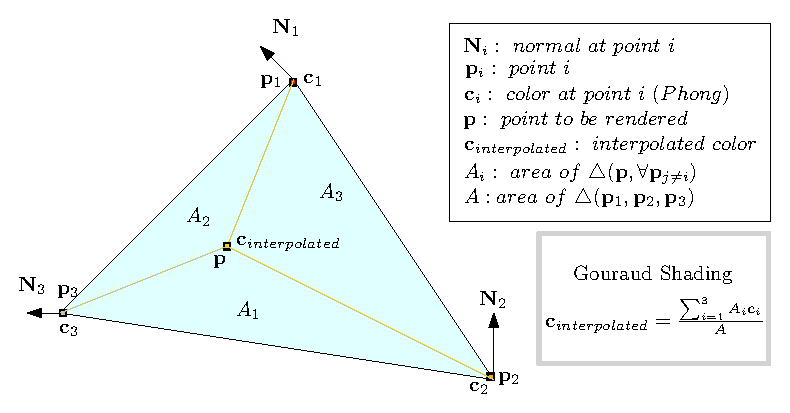
\includegraphics[height=5cm]{Math_lighting/interpolatedColors.eps}
\end{figure}
\end{frame}
%%%%%%%%%%%%%%%%%%%%%%%%%%%%%%%%%%%%%%%%%%%%%%%%%%%%%%%%%



%%%%%%%%%%%%%%%%%%%%%%%%%%%%%%%%%%%%%%%%%%%%%%%%%%%%%%%%%
\begin{frame}[fragile]{구로(Gouraud) 세이딩 예제}

\begin{figure}[h!]
  \centering
    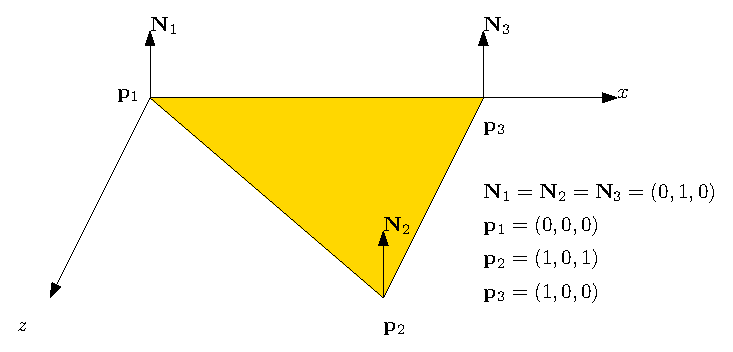
\includegraphics[height=6cm]{Math_lighting/simpleTriangle.eps}
\end{figure}

\end{frame}
%%%%%%%%%%%%%%%%%%%%%%%%%%%%%%%%%%%%%%%%%%%%%%%%%%%%%%%%%



%%%%%%%%%%%%%%%%%%%%%%%%%%%%%%%%%%%%%%%%%%%%%%%%%%%%%%%%%
\begin{frame}[fragile]{구로 세이딩 결과}

\begin{figure}[h!]
  \centering
    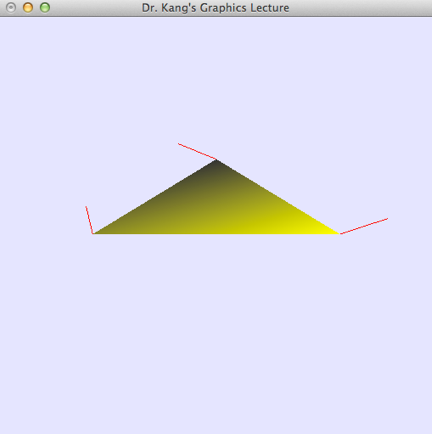
\includegraphics[height=6.5cm]{Math_lighting/normalSetting.png}
\end{figure}

\end{frame}
%%%%%%%%%%%%%%%%%%%%%%%%%%%%%%%%%%%%%%%%%%%%%%%%%%%%%%%%%


